\documentclass{../source/Experiment}

\major{信息工程}
\name{姚桂涛}
\title{小信号调谐放大器}
\expname{小信号调谐放大器}
\stuid{3190105597}
\college{信息与电子工程学院}
\date{\today}
\lab{东4-319}
\course{通信原理实验}
\instructor{金向东、龚淑君}
\grades{}
\exptype{验证性实验}
\partner{叶慷鹏}
\begin{document}
\section{实验目的和要求}
    (1)掌握小信号调谐放大器的工作原理。

    (2)掌握频谱分析仪的基本使用方法。

    (3)掌握调谐放大器电压增益、通频带及选择性的定义、测试及计算方法。

    \section{实验原理}
    小信号调谐放大器广泛用作高频和中频放大器,特别是用在通信接收端的前端电路,其主要目的就是实现对高频小信号的放大。

    小信号调谐放大器的幅频特性:
    \begin{figure}[H]
        \centering
        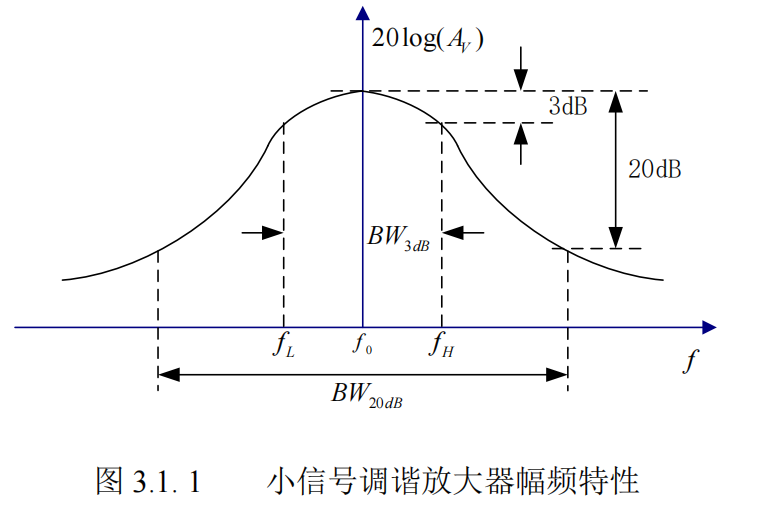
\includegraphics[scale=0.4]{pic/fig1.png}
    \end{figure}

    调谐放大器特性测试采用扫频法,采用带跟踪源的频谱仪进行测试。

    \section{实验电路分析}

    实验电路如图所示。该电路由晶体管 Q3、选频回路二部分组成。本实验中谐振频率接近 10.7MHz,调整 T1的电感量可改变谐振频率。作为双调谐放大器,T1,T2需要同时进行调整。基极偏置电阻 WR2、R17、R18 和射极电阻 R19 决定晶体管的静态工作点。调节可变电阻 WR2 改变基极偏置电阻将改变晶体管的静态工作点,从而可以改变放大器的增益。
    
    通过开关 SW3的切换,可以改变电路形式或选择不同耦合电容。当 SW3 两位拨码开关设成“00”,即都设为“OFF”时,电路就成为单调谐放大器了,信号从 JP5 输出。当 SW3 设成其它状态时,电路为双调谐放大器,切换不同的耦合电容从而改变耦合系数,进而影响电路的选频特性。

    \section{实验设备}
        \begin{enumerate}
            \item 实验办No01 \, 1块
            \item 信号源1台
            \item 双踪示波器1台
            \item 频谱分析仪(含TG)1台
            \item 外用表1台
        \end{enumerate}
        
    \section{实验数据与结果分析}
        \subsection{单调谐小信号放大器实验}
            \subsubsection{晶体管静态工作点调整}
            
            实验中我们通过调整电阻$WR_2$的阻值,使$V_{EQ} = 1.5V$从而测得$I_{EQ}$并使其为$\dfrac{1.5V}{470\Omega} = 3.91mA$
            
            \subsubsection{谐振频率测试}

            选择示波器的【Peak】按钮,读取频率值得到谐振频率。

            但是观察示波器得到的图像可以看到,波形靠近波峰的位置有一个不正常的尖峰,分析可能是由于跟踪源带来的误差导致的,所以此时如果直接用【Peak】按钮测量得到的谐振频率会得到错误的结果。实验中我们于是采用了手动调整测量光标来测量,得到的谐振频率为$10.433MHz$,由于是手动测量,所以结果含有误差。
            
            \subsubsection{谐振增益测试}

            由上图测量结果,功率峰值为$2.15dbm$,输入功率为$-20dbm$,可以得到功率增益为$G = P_0 - P_1 = 22.15dbm$
            
            \subsubsection{通带测试}

            实验中我们小组采用方法二进行测量,即采用频谱仪自带的带宽测量功能,选择【3】【dB】测量得到$3dB$带宽为$BW_{3dB} = 2.0666MHz$
            
            \subsubsection{选择性测试}

            实验中测得左边$-20dB$频率为$4.966MHz$,而无法直接测得右边的$-20dB$频率,所以我们将测得的谐振频率减去左边的$-20dB$频率并乘2得到近似带宽。
            $$BW_{20dB} = 10.433 - 4.966)$$
            
            \subsubsection{静态工作点对谐振放大器增益和带宽的影响}
            
        \subsection{双调谐小信号放大器实验}
            
            \subsubsection{耦合状态观测}
            
            \subsubsection{谐振增益测试}
            
            \subsubsection{通带测试}
            
            \subsubsection{选择性测试}
            
            \subsubsection{静态工作点对谐振放大器增益和带宽的影响}

    \section{思考题}
	    \subsection{高频小信号放大器的主要技术指标有哪些?}
	
        谐振频率($f_0$)、谐振增益($A_{V0}$)、通频带($BW_{3dB}$)、增益带宽积($A_{V0}BW_{3dB}$)、选择性($K_{V0.1}$)
        
        \subsection{单级单调谐放大器的电压增益与那些因素有关?当谐振回路中的并联电阻R变化时,增益及带宽将怎样变化?当谐振放大器的静态工作点变化时,增益及带宽将怎样变化?}
        
        单级单调谐放大器的电压增益与三极管的正向传输导纳、负载导纳、谐振回路导纳、接入系数等有关,也与晶体管的电流放大系数、谐振电路的品质因数、温度等有关。
        
        若增大R,电压增益变大,带宽变小(增益带宽积基本不变)。

        随着静态工作电流变大,增益增加及带宽基本不变。

        \subsection{回路的谐振频率和那些参数有关?如何判断谐振回路处于谐振状态?}
	
	    主要与$L$、$C$有关;当功率增益达到最大时即处于谐振状态。
	
\end{document}